%\pagestyle{empty}

\IfSubStr*{\jobname}{print}{
	\thispagestyle{empty}
	{
	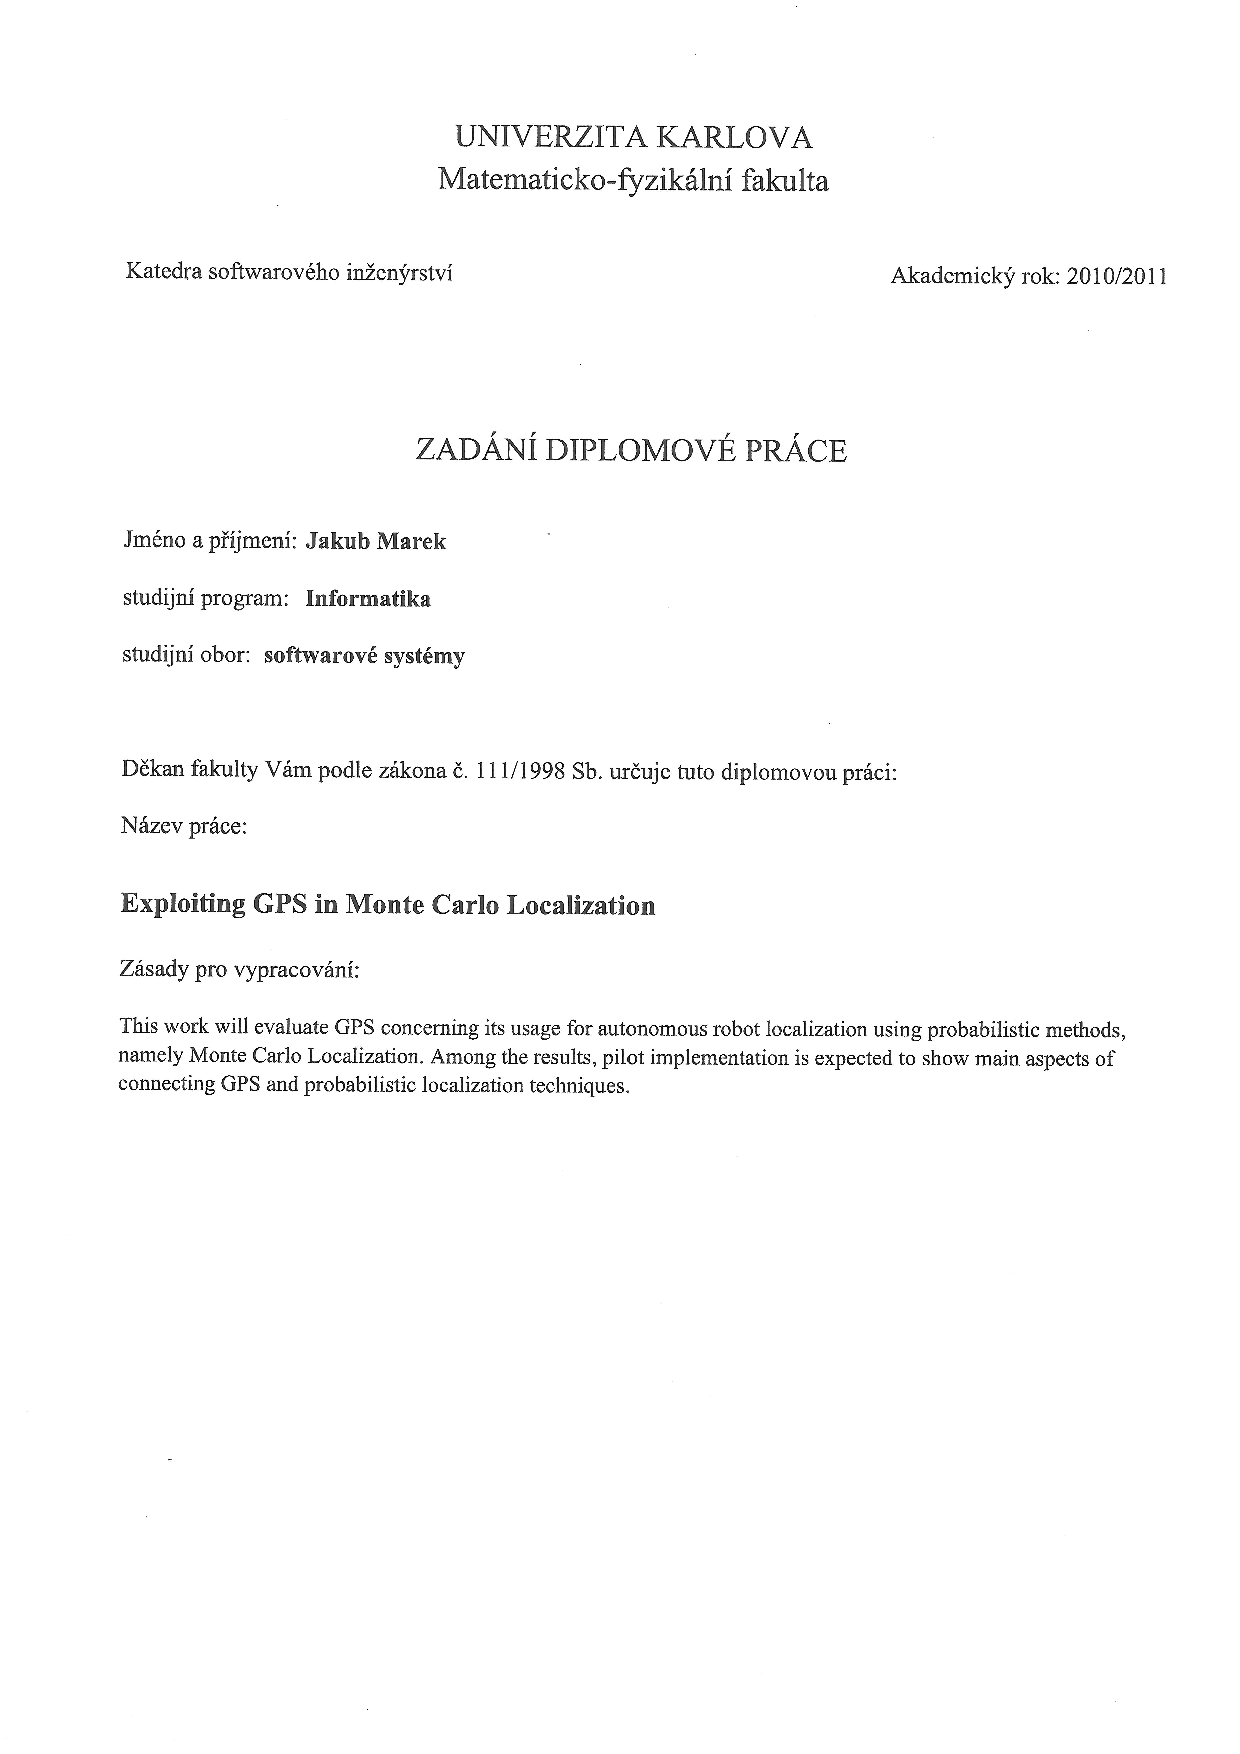
\includepdf{img/assignment-front.pdf}
	}
	\thispagestyle{empty}
	{
	\centering
	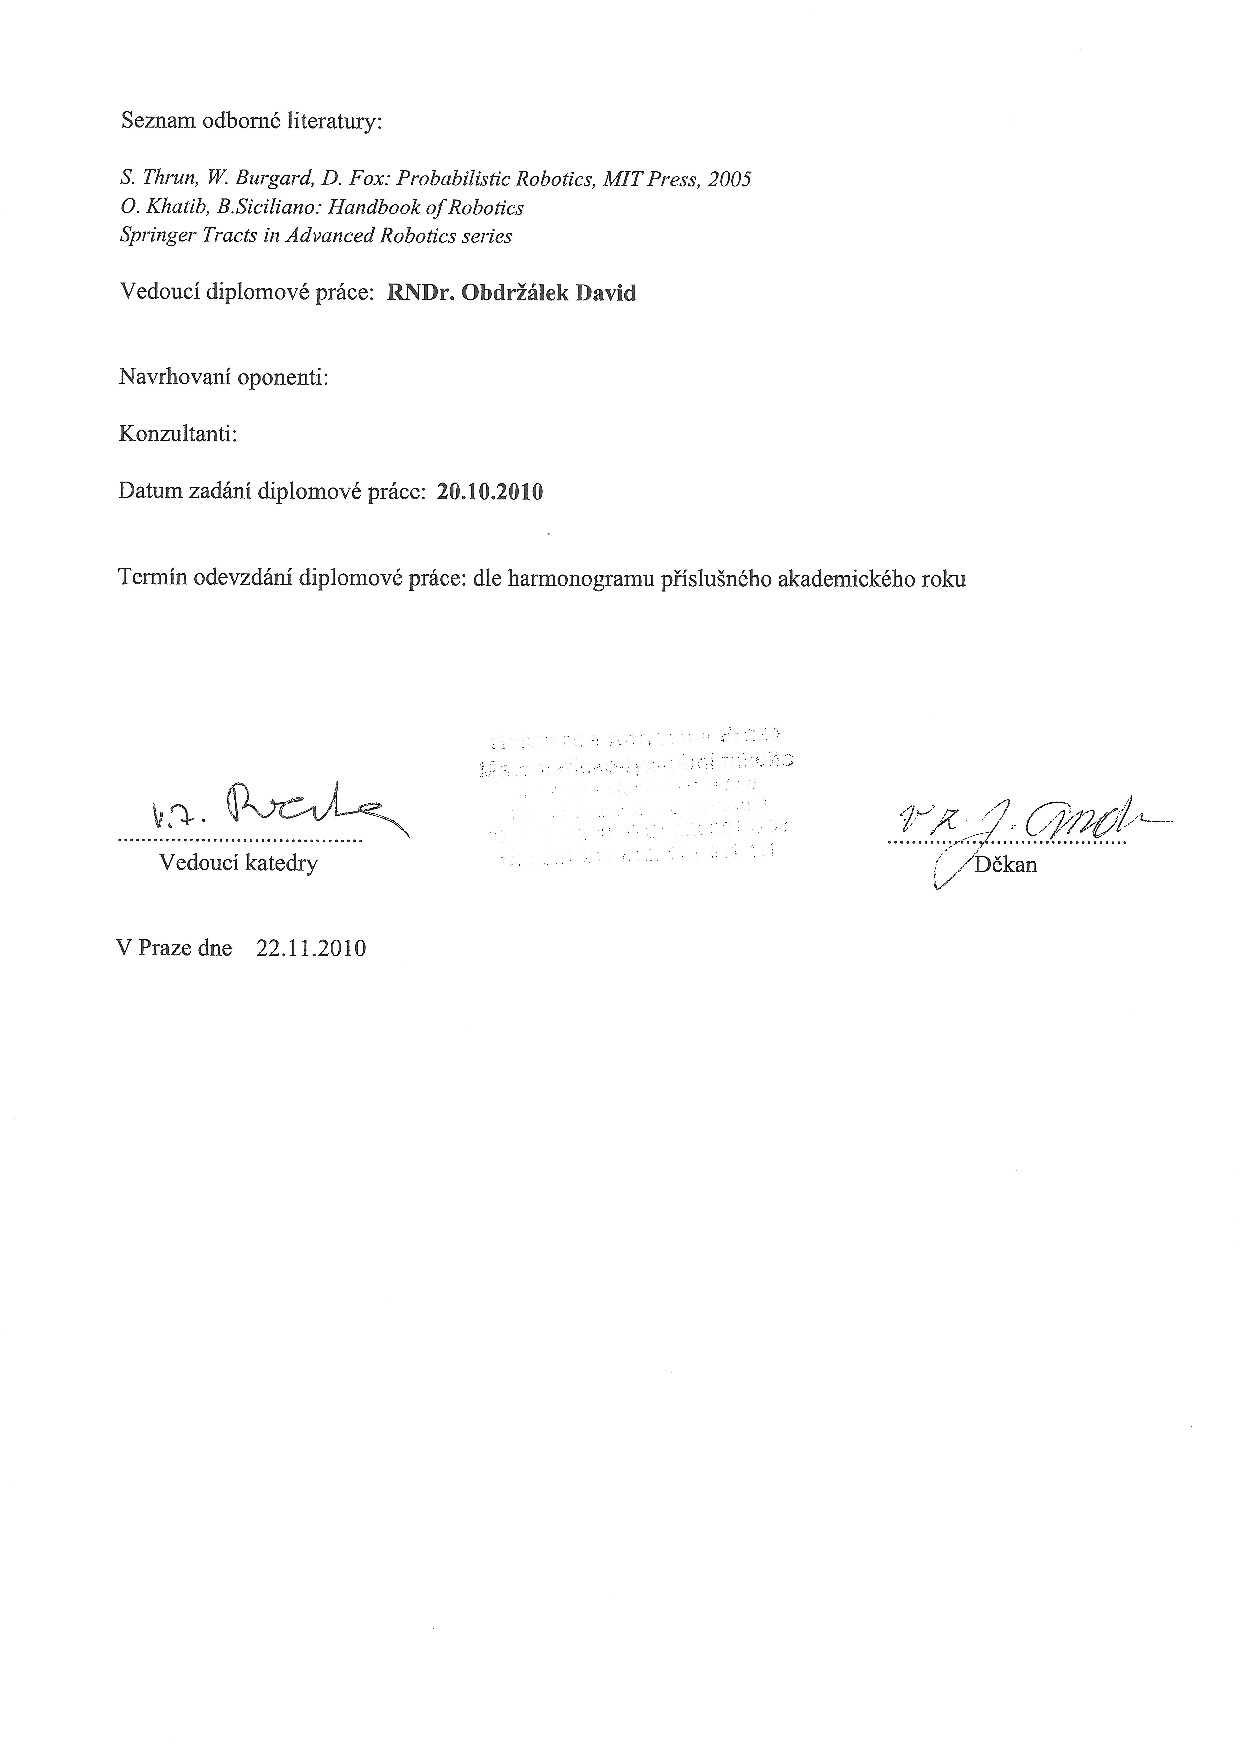
\includepdf{img/assignment-back.pdf}
	}
	\newpage
}{}

\vspace{10mm} 

Thank you.

Also I would like to thank to the team of Roboauto Karlík for letting me
record valuable real life data from their robot.

\newpage

\vspace*{\fill}
I declare that I carried out this master thesis independently, and only with the cited
sources, literature and other professional sources.

I understand that my work relates to the rights and obligations under the Act No.
121/2000 Coll., the Copyright Act, as amended, in particular the fact that the Charles
University in Prague has the right to conclude a license agreement on the use of this
work as a school work pursuant to Section 60 paragraph 1 of the Copyright Act.

\vspace{10mm} 
\noindent In~Prague, \today\hspace{\fill}Jakub Marek\\
\newpage

\tableofcontents*
\newpage

\noindent
Title: \thetitle\\
Author: \theauthor\\
Department / Institute: Department of Software Engineering\\
Supervisor of the master thesis: RNDr. David Obdržálek, Department of Software Engineering\\

\noindent Abstract: 
\noindent Keywords: robotics, gps, pseudorange, localization

\vspace{25mm}

%\begin{otherlanguage}{czech}
\noindent
Název práce: Použití GPS v Monte Carlo lokalizaci\\
Autor: \theauthor\\
Katedra / Ústav: Katedra softwarového inženýrství\\
Vedoucí diplomové práce: RNDr. David Obdržálek, Katedra softwarového inženýrství\\

\noindent Abstrakt: 

\noindent Klíčová slova: robotika, gps, pseudorange, lokalizace
%\end{otherlanguage}

\newpage

%\pagestyle{plain}
%\setcounter{page}{1}
